\chapter[Recursão]{Recursão}

\section{Introdução}\label{sec1.1}


A decomposição é umas das quatro habilidades principais da Pensamento Computacional. A decomposição é uma habilidade que consiste em dividir um problema complexo em partes menores que são mais fáceis de entender. 

A recursão pode ser entendida como uma caso particular de decomposição. Na recursão, um problema complexo é decomposto em parte(s) menores do mesmo problema. Nós podemos usar a recursão para definir sequências, funções, conjuntos e algoritmos.  

O processo de recursão aplicado a um problema pode ser definido da seguinte maneira:

\begin{itemize}
    \item Se um problema pode ser resolvido diretamente, então resolva-o.
    \item Caso contrário, reduza o problema em uma ou mais instâncias menores do mesmo problema.
\end{itemize}



\section{Definições recursivas de funções}\label{sec1.2}

Considere o seguinte exemplo: 

\begin{exemplo}
Uma linha de quadrados é construída usando palitos de fósforo, como mostrado na figura abaixo.


\begin{figure}[htbp]
\centering
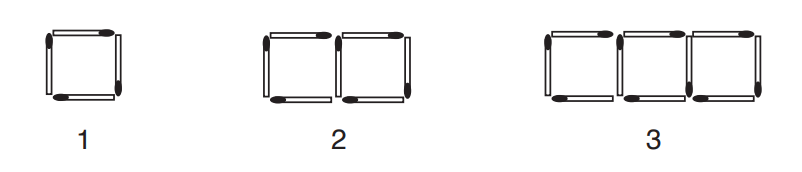
\includegraphics[width=.9\textwidth]{images/fosforos.png}
\label{fig::palitos}
\caption{Quadrados de palitos} 
7

\end{figure}

Quantos palitos são necessários para a construção de uma linha de $n$ quadrados? 

\end{exemplo}

Seja $f(n)$ o número de palitos necessários para construir uma linha de $n$ quadrados.

A definição recursiva pode ser separada em dois casos:

\begin{itemize}
    \item \textbf{Passo Base:} Especifica o valor da função para o menor valor.
    \item \textbf{Passo Recursivo:} Apresenta uma regra para resolver o problema maior a partir de casos menores do mesmo problema.
\end{itemize}

Observando a Figura \ref{fig::palitos}, notamos que toda vez que retiramos 3 palitos de uma linha com $n$ quadrados, obtemos uma linha com $n-1$ quadrados e com 4 palitos obtemos uma linha com 1 quadrado. Acabamos de especificar as regras para tratar os casos complexos e os casos simples.

A definição recursiva da função $f(n)$ é:

\begin{itemize}
    \item \textbf{Passo Base:} $f(1) = 4$
    \item \textbf{Passo Recursivo:} $f(n) = f(n-1) + 3$
\end{itemize}

\begin{exemplo}
João trabalha no supermercado, e seu gerente pediu que ele empilhasse latas de ervilhas como na figura abaixo.


\begin{figure}[htbp]
\centering
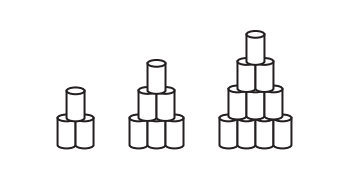
\includegraphics[width=.9\textwidth]{images/Latas.png}
\label{fig::palitos}
\caption{Pilha de latas no supermercardo}
\end{figure}


Proponha uma definição recursiva para o número de latas necessárias para construir uma pilha de latas nesse formato com altura de $n$ latas. 
\end{exemplo}

Seja $p(n)$ o número de latas necessárias para construir uma pilhas de latas no formato acima com uma altura $n$. 

Novamente, precisamos identificar o(s) caso(s) mais simples e como reduzir uma caso complexo em um ou mais casos simples do mesmo problema. A pilha mais simples de ser construída é a pilha de altura 1. Observe também que uma pilha de latas com altura $n$ possui $n$ latas na base. A remoção dessas $n$ latas da base reduz a altura da pilha de latas em 1 unidade.  

Dessa maneira, a definição recursiva para $p(n)$ será:

\begin{itemize}
    \item \textbf{Passo Base:} $p(1) = 1$
    \item \textbf{Passo Recursivo:} $p(n) = p(n-1) + n$
\end{itemize}


\begin{exemplo}
Imagine que você queira construir uma parede de tijolos de comprimento $n$ e altura 2 com tijolos com o comprimento 1 e altura 2 que podem ser rotacionados. Calcule de quantos padrões podemos construir uma parede com comprimento $n$ \footnote{\href{https://onlinejudge.org/index.php?option=com_onlinejudge&Itemid=8&page=show_problem&problem=841}{Problema UVA 900}}.

\begin{figure}[!htbp]
\label{fig::tijolos}
\begin{center}
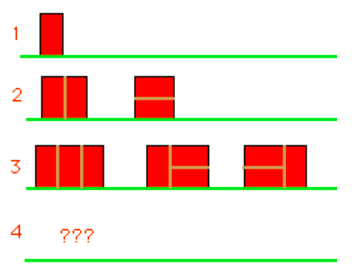
\includegraphics[scale=0.7]{images/pattern.png} 
\end{center}
\caption{Padrões de construções da parede com tijolos 1 x 2}

\end{figure}

\end{exemplo}

Seja $t(n)$ o número de maneira de construir uma parede $n \times  2$ de comprimento $n$ com altura 2 usando apenas o tijolo 2x1 que podem ser rotacionados.

Primeiramente, vamos investigar como reduzir esse problema para obter instâncias menores do mesmo problema. Observando os padrões de construção da parede 3 x 2 na Figura \ref{fig::tijolos}, podemos concluir que os últimos tijolos podem ser colocado de duas maneiras diferente:


\begin{itemize}

\item O último tijolo em pé
    
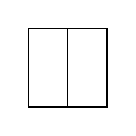
\begin{tikzpicture}
\draw [draw=black] (0,0) rectangle (0.5,1);
\draw [draw=black] (0.5,0) rectangle (1,1);
\end{tikzpicture}
,
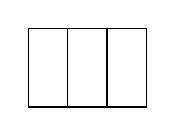
\begin{tikzpicture}
\draw [draw=black] (0,0) rectangle (0.5,1);
\draw [draw=black] (0.5,0) rectangle (1,1);
\draw [draw=black] (1,0) rectangle (1.5,1);
\end{tikzpicture}

\item Os dois últimos tijolos deitados

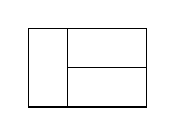
\begin{tikzpicture}
\draw [draw=black] (0,0) rectangle (0.5,1);
\draw [draw=black] (0.5,0) rectangle (1.5,0.5);
\draw [draw=black] (0.5,0.5) rectangle (1.5,1);
\end{tikzpicture}

\end{itemize}

No primeiro caso, removendo o último tijolo, reduzimos o comprimento da parede em 1 unidade. No segundo caso, removendo os dois últimos tijolos, reduzimos o comprimento da parede em 2 unidades.


Neste problema, os problemas que podem ser resolvidos diretamente sem o uso das regras acima como caso simples. Observe, novamente na Figura \ref{fig::tijolos}, as paredes de comprimento 1 e 2 podem ser resolvidas diretamente. 


Dessa maneira, a definição recursiva para $t(n)$ será:

\begin{itemize}
    \item \textbf{Passo Base:} $t(1) = 1$
    \item \textbf{Passo Base:} $t(2) = 2$
    
    \item \textbf{Passo Recursivo:} $t(n) = t(n-1) + t(n-2)$
\end{itemize}

\begin{exemplo}
Você passa em uma loja perto de sua casa e vê a seguinte oferta: Uma garrafa de chococola para cada 3 garrafas vazias devolvidas. Você decide comprar algumas garrafas de cola nessa loja, agora você quer saber quantas garrafas de chococola você pode beber se você aproveitar essa promoção sempre que possível?\footnote{\href{https://onlinejudge.org/index.php?option=onlinejudge&Itemid=8&category=226&page=show_problem&problem=2999}{UVA 11877 - The Coco-Cola Store}}
\end{exemplo}

A Figura \ref{fig::chococola} mostra quantas garrafas de chococola você pode beber comprando inicialmente 8 garrafas de chococola.


\begin{figure}[!htbp]

\label{fig::chococola}
\begin{center}
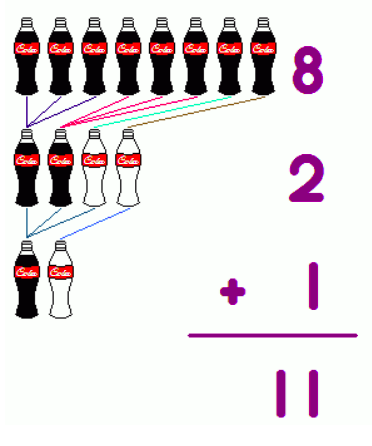
\includegraphics[scale=0.5]{images/cola.png} 
\end{center}
\caption{Promoção chococola}
\end{figure}

Neste problema, utilizaremos a variável $n$ para guardar o número de garrafas cheias e a variável $m$ para guardar o número de garrafas vazias. 

O nosso problema é encontrar uma definição recursiva para a função $cola(n,m)$ que devolve o número de garrafas que você pode beber aproveitando essa promoção sempre que possível considerando que você tem inicialmente $n$ garrafas cheias e $m$ garrafas vazias.

Agora, precisamos encontrar uma maneira genérica para reduzir uma entrada do problema para uma entrada mais simples do mesmo problema. Considere que você tem 5 garrafas cheias  e 3 garrafas vazias, você pode beber 5 garrafas cheias. Depois, você vai ficar com 8 garrafas vazias. Utilizando a promoção, você pode conseguir mais 2 garrafas cheias e 2 vazias. 

Os casos mais simples desse problema ocorre quando $n+m < 3$. Nestes casos, você pode beber apenas $n$ garrafas de chococola.


Dessa maneira, a definição recursiva para $cola(n,m)$ será:

\begin{itemize}
    \item \textbf{Passo Base:} $cola(n,m) = n$, se $n+m < 3$
    \item \textbf{Passo Recursivo:} $cola(n,m) = n + coca( \lfloor (n+m)/3 \rfloor , (n+m) \mod 3)$
\end{itemize}

\begin{exemplo}
De quantas maneiras distintas $n$ objetos distintos podem ser organizados em uma sequência de tamanho $n$?


\begin{itemize}
    \item 1 objeto pode ser organizado em uma sequência de tamanho 1 de 1 maneira: A;
    \item 2 objetos podem ser organizados em uma sequência de tamanho 2 de 2 maneiras: BA, AB;
    \item 3 objetos podem ser organizados em uma sequência de tamanho 3 de 6 maneiras: BCA, CBA, ACB, CAB, ABC e BAC;
\end{itemize}

\end{exemplo}

Encontraremos a definição recursiva para a função $p(n)$ que devolve o número de maneiras que podemos organizar $n$ objetos distintos em uma sequência de tamanho $n$.

O caso mais simples desse problema ocorre quando temos apenas 1 objeto distinto para organizar em uma sequência de tamanho 1. Novamente, precisamos descobrir uma maneira de reduzir um problema complexo em uma versão mais simples do mesmo problema. Propositalmente, as sequências de tamanho 3 foram listadas de uma maneira peculiar. Começamos listando as sequências terminadas em A, depois B, e assim por diante. Observe que se temos $n$ objetos distintos, temos $n$ opções para o último objeto. Toda vez que utilizamos 1 objeto na última posição, temos que resolver o problema de organizar $n-1$ objetos distintos em uma sequência de tamanho $n-1$.



Dessa maneira, a definição recursiva para $p(n)$ será:

\begin{itemize}
    \item \textbf{Passo Base:} $p(1) = 1$
    \item \textbf{Passo Recursivo:} $p(n) = n * p(n-1)$
\end{itemize}


\begin{exemplo}
De quantas maneiras distintas $n$ objetos distintos podem ser organizados em uma sequência de tamanho $k$?


\begin{itemize}
    \item 4 objetos (A,B,C e D) podem ser organizados em uma sequência de tamanho 2 de  12 maneiras: BA, CA, DA, AB, CB, DB, AC, BC, DC, AD, BD e CD. 
    ;
\end{itemize}

\end{exemplo}


Encontraremos a definição recursiva para a função $p(n,k)$ que devolve o número de maneiras que podemos organizar $n$ objetos distintos em uma sequência de tamanho $k$.


O caso mais simples desse problema ocorre quando temos apenas $n$ objeto distinto para organizar em uma sequência de tamanho 1, obtendo $n$ maneiras distintas. 

Novamente, precisamos descobrir uma maneira de reduzir um problema complexo em uma versão mais simples do mesmo problema. Propositalmente, as sequências de tamanho 3 foram listadas de uma maneira peculiar. Começamos listando as sequências terminadas em A, depois B, e assim por diante. Observe que se temos $n$ objetos distintos, temos $n$ opções para o último objeto. Toda vez que utilizamos 1 objeto na última posição, temos que resolver o problema de organizar $n-1$ objetos distintos em uma sequência de tamanho $k-1$.


Dessa maneira, a definição recursiva para $p(n)$ será:

\begin{itemize}
    \item \textbf{Passo Base:} $p(n, 1) = n$
    \item \textbf{Passo Recursivo:} $p(n,k) = n * p(n-1, k-1)$
\end{itemize}

Utilizando a definição acima, temos que:

\begin{itemize}
    \item p(4,2) = 4 * p(3,1) = 4 * 3 = 12
\end{itemize}


% \begin{exemplo}
% Quantos triângulos em pé (tamanhos variados)
%   podemos encontrar em uma grade triangular com
%   altura $n$?
  
% \begin{center}
%     \begin{tikzpicture}
%     \foreach \i in {0,1,2,3,4} {
%       \draw (0 + 0.5*\i, \i * 0.5 * \sqrtofthree) -- (4 - 0.5*\i, \i * 0.5 * \sqrtofthree);
%       \draw (0:\i) -- (60:\i);
%       \draw[xshift=4cm] (180:\i) -- (120:\i);
%     }
%     \end{tikzpicture}
%     \qquad
%     \begin{tikzpicture}
%     \fill[yellow!80] (0,0) -- (3,0) -- (1.5,3*0.5*\sqrtofthree);
%     \fill[green!80] (1.5,0.5*\sqrtofthree) -- (3.5,0.5*\sqrtofthree) -- (2.5,3*0.5*\sqrtofthree);
%     \foreach \i in {0,1,2,3,4} {
%       \draw (0 + 0.5*\i, \i * 0.5 * \sqrtofthree) -- (4 - 0.5*\i, \i * 0.5 * \sqrtofthree);
%       \draw (0:\i) -- (60:\i);
%       \draw[xshift=4cm] (180:\i) -- (120:\i);
%     }
%     \end{tikzpicture}
%   \end{center}

% Destacamos dois triângulos de tamanhos variados encontrados em um triângulo de altura 4.

% \end{exemplo}  

% Seja $t(n)$ o número de triângulos em pé de tamanho variados que podemos encontrar em um grade triangulas com altura $n$.

% Para uma grade de altura $n = 1$, temos $t(1) = 1$ triângulo

% \begin{center}
%     \begin{tikzpicture}
%       \draw (0,0) -- (2,0) -- (1,2*0.5*\sqrtofthree) -- cycle;
%     \end{tikzpicture}
%   \end{center}
  
% Para uma grade de altura $n = 2$, temos $t(2) = 4$ triângulo.

% \begin{itemize}
%   \item 2 com o vértice superior coincidindo com o vértice superior do maior triângulo.
%   \item 2 outros triângulos com o vértice superior diferente do vértice superior do maior triângulo.
% \end{itemize}


% \begin{center}

% \begin{tabular}{ll}

%      \begin{tikzpicture}
%       \foreach \i in {0,1,2} {
%         \draw (0 + 1*\i, \i * 1 * \sqrtofthree) -- (4 - 1*\i, \i * 1 * \sqrtofthree);
%         \draw (0:2*\i) -- (60:2*\i);
%         \draw[xshift=4cm] (180:2*\i) -- (120:2*\i);
%       }
%       \draw[fill=blue!80] (1,\sqrtofthree) -- (3,\sqrtofthree) -- (2,2*\sqrtofthree) -- cycle;
%       \draw[ultra thick, red!80] (0,0) -- (4,0) -- (2, 2*\sqrtofthree) -- cycle;
%       \draw[ultra thick, red!80] (0,0) -- (4,0) -- (2, 2*\sqrtofthree) -- cycle;
%     \end{tikzpicture}
% &
%          \begin{tikzpicture}
%       \foreach \i in {0,1,2} {
%         \draw (0 + 1*\i, \i * 1 * \sqrtofthree) -- (4 - 1*\i, \i * 1 * \sqrtofthree);
%         \draw (0:2*\i) -- (60:2*\i);
%         \draw[xshift=4cm] (180:2*\i) -- (120:2*\i);
%       }
     
%       \draw[fill=green!80] (0,0) -- (2,0) -- (1,\sqrtofthree) -- cycle;     
%       \draw[fill=yellow!80] (2,0) -- (4,0) -- (3,\sqrtofthree) -- cycle;
      
%     \end{tikzpicture}\\
% \end{tabular}
%   \end{center}

% Para uma grade triangular de altura n = 3:






%      \begin{tikzpicture}
%       \foreach \i in {0,1,2} {
%         \draw (0 + 1*\i, \i * 1 * \sqrtofthree) -- (4 - 1*\i, \i * 1 * \sqrtofthree);
%         \draw (0:2*\i) -- (60:2*\i);
%         \draw[xshift=4cm] (180:2*\i) -- (120:2*\i);
%       }
%       \draw[fill=blue!80] (1,\sqrtofthree) -- (3,\sqrtofthree) -- (2,2*\sqrtofthree) -- cycle;
%       \draw[ultra thick, red!80] (0,0) -- (4,0) -- (2, 2*\sqrtofthree) -- cycle;
%       \draw[ultra thick, red!80] (0,0) -- (4,0) -- (2, 2*\sqrtofthree) -- cycle;
%     \end{tikzpicture}


\begin{exemplo} Ao subir a escada de seu prédio, José às vezes sobe dois degraus de uma vez e às vezes sobe um de cada vez. Sabendo que a escada tem $n$ degraus, de quantas maneiras diferentes José pode subir a escada? 

\end{exemplo}

Primeiramente, vamos pensar nos casos menores:

\begin{itemize}
    \item Uma escada de 1 degrau, podemos subir as escadas de 1 maneira (1).
    \item Uma escada de 2 degrau, podemos subir as escadas de 2 maneiras (1+1,2).
    \item Uma escada de 3 degraus, podemos subir as escadas de 3 maneiras (1+1+1,1+2,2+1).
\end{itemize}


Seja $f(n)$ número de maneira de subir uma escada de $n$ degraus. O primeiro passo para subir uma escada de n degraus pode ser dado de duas maneiras:

\begin{itemize}
    \item Se você subir apenas um degrau, então teremos $f(n-1)$ maneiras de subir uma escada de $n-1$ degraus.
    \item Se você subir dois degraus, então teremos $f(n-2)$ maneiras de subir uma escada de $n-2$ degraus.
\end{itemize}

Consideramos como case mais simples, os casos que não precisamos usar a regra acima para resolver o problema.


Dessa maneira, a definição recursiva para $f(n)$ será:

\begin{itemize}
    \item \textbf{Passo Base:} $f(1) = 1$
    \item \textbf{Passo Base:} $f(2) = 2$
    
    \item \textbf{Passo Recursivo:} $f(n) = f(n-1) + f(n-2)$
\end{itemize}

% \begin{exemplo}
% Quantas são as sequências de $n$ termos pertencentes a \{0,1\}, que possuem um quantidade ímpar de termos iguais a 0?

% Exemplos:

% \begin{itemize}
% \item Sequências de tamanho 1: 1 \{ 0 \} 
% \item Sequências de tamanho 2: 2 \{ 01 e 10 \}
% \item Sequências de tamanho 3: 4 \{ 000,011,101,110 \}


% \end{itemize}

% \end{exemplo}



% Seja $f(n)$ o número de sequências de $n$ termos 0 e 1 com uma quantidade ímpar de termos iguais a 0. Novamente, precisamos encontrar uma maneira de reduzir o problema para encontrar uma versão mais fácil. Se uma sequência de $n$ termos tem uma quantidade ímpar de zeros então:
% \begin{itemize}
%     \item se a sequência começa com  1 será seguida por uma sequência de $n-1$ termos com uma quantidade ímpar de zeros.
    
%     \item se a sequência começar com 0 seguido por um sequência de $n-1$ termos com um número par de zeros.
% \end{itemize}

% No segundo caso, temos um problema diferente do problema original, então podemos fazer uma redução maior.

% \begin{itemize}
%     \item se a sequência começa com  1 será seguida por uma sequência de $n-1$ termos com uma quantidade ímpar de zeros.
    
%     \item se a sequência $b_1b_2 \ldots b_n$ começa com 0 então podemos dividir essa sequência em duas partes:
%         \begin{itemize}
%             \item $b_1 \ldots b_k$ 
%             \item $b_k \ldots b_n$
%         \end{itemize}
%     tal que ambas tem uma quantidade ímpar de zeros e ambas começam e terminam com zeros.
    
% \end{itemize}


\section{Definições recursivas de conjuntos}

Muitos conjuntos podem ser definidos com o auxílio da recursão. 

\begin{exemplo}
Dado um alfabeto $\Sigma$, encontre uma definição do conjunto de todas as palavras formada no alfabeto $\Sigma$ com tamanho $n$, denotado por $\Sigma^n$. Por exemplo, se $\Sigma = \{a,b,c\}$ então

\begin{itemize}
    \item $\Sigma^0 = \{ \varepsilon \}$, onde $\varepsilon$ denota a string vazia.
    \item $\Sigma^1 = \{ a,b,c \}$
    
    \item $\Sigma^2 = \{ aa,ab,ac, ba,bb,bc, ca,cb,cc \}$
    
\end{itemize}

\end{exemplo}
 
Naturalmente, o caso mais simples acontece quando $n = 0$. Novamente, precisamos encontrar uma maneira de reduzir o problema, note que em uma palavra de tamanho $n$, o primeiro caractere é um símbolo de $\Sigma$ seguido de uma palavra de tamanho $n-1$.


Dessa maneira, a definição recursiva para $\Sigma^n$ será:

\begin{itemize}
    \item \textbf{Passo Base:} $\Sigma^0 = \{ \varepsilon\}$
    
    \item \textbf{Passo Recursivo:} $\Sigma^n = \{ ax : a \in \Sigma, x \in \Sigma^{n-1}\}$
\end{itemize}


\begin{exemplo}
Dado um alfabeto $\Sigma$, encontre uma definição do conjunto de todas as palavras formada no alfabeto $\Sigma$ com tamanho $n$, denotado por $\Sigma^*$. Por exemplo, se $\Sigma = \{a,b\}$ então $\Sigma^* = \{\varepsilon,a,b,aa,ab,ba,bb,\ldots\}$
\end{exemplo}

Neste caso, a definição recursiva indica uma regra para a construção de novos elementos a partir de elementos anteriores. A definição recursiva de $\Sigma^*$ é :

\begin{itemize}
    \item \textbf{Passo Base:} $\varepsilon \in \Sigma^*$
    
    \item \textbf{Passo Recursivo:} Se $x \in \Sigma^*$ então $ax \in \Sigma^*, \forall a \in \Sigma$ 
\end{itemize}



\begin{exemplo}
Uma palavra é dita palíndroma quando ela pode ser lida da esquerda para a direita ou vice-versa sem alteração na palavra: osso, ana, renner.

Dado um alfabeto $\Sigma$, encontre uma definição do conjunto de todas as palavras palíndroma formada no alfabeto $\Sigma$ com tamanho $n$ , denotado por $\Sigma^n$. Seja $Pal(\Sigma, n)$ o conjunto de todas as palavras palíndroma no alfabeto $\Sigma$ de tamanho $n$. Por exemplo, se $\Sigma = \{a,b,c\}$ então

\begin{itemize}
    \item $Pal(\Sigma, 0) = \{ \varepsilon \}$, onde $\varepsilon$ denota a string vazia.
    \item $Pal(\Sigma, 1) = \{ a,b,c \}$
    
    \item $Pal(\Sigma,2) = \{ aa,bb,cc \}$
    
\end{itemize}

\end{exemplo}
 


Primeiramente, vamos investigar como reduzir esse problema. Em palavra palíndroma de tamanho $n$, o primeiro e o último caractere devem ser iguais e palavra obtida pela remoção desses caracteres deve ser palíndroma. Note que este processo pode ser realizado até chegar em um string vazia no caso da palavra osso ou em uma string de tamanho 1 no caso da palavra ana.


 Dessa maneira, a definição recursiva para $Pal(\Sigma, n)$ será:

\begin{itemize}
    \item \textbf{Passo Base:} $Pal(\Sigma,0) = \{ \varepsilon\}$
    
    \item \textbf{Passo Base:} $Pal(\Sigma,1) = \Sigma $
    
    \item \textbf{Passo Recursivo:} $Pal(\Sigma,n) = \{ axa : a \in \Sigma, x \in Pal(\Sigma,n-2)\}$
\end{itemize}


\begin{exemplo}
Dado um alfabeto $\Sigma$, encontre uma definição do conjunto de todas as palavras palíndroma formada no alfabeto $\Sigma$. Por exemplo, se $\Sigma = \{a,b\}$ então $Pal(\Sigma) = \{ \varepsilon, a, b, aa, bb, aba, aaa, bab, bbb, \ldots\}$
\end{exemplo}
 
Note que o conjunto $Pal(\Sigma)$ não é finito. Neste caso, a definição recursiva vai apresentar uma regra para construção de novas palavras palíndromas a partir de palavras palíndromas prévias.

A definição recursiva de $Pal(\Sigma)$ é :

\begin{itemize}
    \item \textbf{Passo Base:} $\varepsilon \in Pal(\Sigma)$
    
    \item \textbf{Passo Recursivo:} Se $x \in Pal(\Sigma)$ então $axa \in Pal(\Sigma), \forall a \in \Sigma$ 
\end{itemize}



\begin{exemplo}
Dado um cojunto $S$, o conjunto de todos os subconjuntos de $S$ será denotado por $\mathcal{P}(S)$. Por exemplo,

\begin{itemize}
    \item $\mathcal{P}(\emptyset) = \{\emptyset \}$
    \item $\mathcal{P}(\{1\}) = \{\emptyset , \{1\}\}$
    \item $\mathcal{P}(\{1,2\}) = \{\emptyset,\{2\},\{1\}, \{1,2\}\}$
    \item $\mathcal{P}(\{1,2,3\}) = \{\emptyset,\{2\},\{1\}, \{1,2\},\{3\},\{2,3\},\{1,3\},\{1,2,3\}\}$
    
\end{itemize}

\end{exemplo}

Primeiramente, vamos tentar pensar em como reduzir esse problema. Note que os subconjuntos de cada conjunto foram listados de maneira particular para facilitar enxergar o padrão de formação do conjunto $\mathcal{P}(S)$. Precisamos fazer duas observações importantes sobre subconjuntos de $\mathcal{P}(S \cup \{x\}\})$:

\begin{itemize}
    \item Todo subconjunto de $S$ é um subconjunto de $S \cup \{x\}$
    \item Todo subconjunto de $S$ unido com o elemento x é um subconjunto de $S \cup \{x\}$.
\end{itemize}

Com essas duas observações, podemos definir recursivamente $\mathcal{P}(S)$ da seguinte maneira:

\begin{itemize}
    \item \textbf{Passo Base:} $\mathcal{P}(\emptyset) = \{\emptyset\}$
    \item \textbf{Passo Recursivo:} $\mathcal{P}(S \cup \{x\}) = \mathcal{P}(S) \cup \{ X \cup \{x\} | X \subseteq  \mathcal{P}(S)\}$
\end{itemize}

\section{Definições recursivas de operações}

Até o momento, definimos de maneira recursiva funções e conjunto. Nesta seção, vamos definir operações sobre conjuntos definidas de maneira recursiva. Os números naturais são um exemplo de uma estrutura definida de maneira recursiva:

\begin{itemize}
    \item \textbf{Passo Base:} $0 \in \mathbb{N}$
    \item \textbf{Passo Recursivo:} Se $x \in \mathbb{N}$ então $x+1 \in \mathbb{N}$
\end{itemize}



\begin{exemplo}
Dado dois números naturais $a$ e $n$, $a^n$ é o resultado da multiplicação de $n$ cópias de $a$. Por exemplo,

\begin{itemize}
    \item $2^0 = 1$
    \item $2^1 = 2$
    \item $2^2 = 2*2 = 4$
    \item $2^3 = 2*2*2 = 8$
\end{itemize}
\end{exemplo}


Novamente, precisamos descobrir uma maneira de reduzir um problema mais complexo em uma instância mais simples do mesmo problema. Observe que $2^3$ pode ser escrito como $2^2 * 2$. O mesmo vale para todo expoente, ou seja, $a^{n+1}$ pode ser escrito como $a^{n}*a$.



Dessa maneira, a definição recursiva para $a^n$ será:

\begin{itemize}
    \item \textbf{Passo Base:} $a^0 = 1$
    \item \textbf{Passo Recursivo:} $a^{n+1} = a^{n} * a$
\end{itemize}


\begin{exemplo}
Dado uma palavra $x \in \Sigma^*$, defina recursivamente a função $l : \Sigma^* \to \mathbb{N}$ tal que $l(x)$ devolve o tamanho da palavra $x$.
\end{exemplo}


A definição recursiva da função $l$ será:

\begin{itemize}
    \item \textbf{Passo Base:} $l(\varepsilon) = 0$
    \item \textbf{Passo Recursivo:} se $x \in \Sigma^*$ e $a \in \Sigma$ então $l(xa) = l(x) + 1$
\end{itemize}


\begin{exemplo}
Dado duas palavra $x \in \Sigma^*$ e $y \in \Sigma^*$, defina recursivamente a operação $x \circ y$ representando a concatenação das duas palavras $x$ e $y$. Por exemplo,

\begin{itemize}
    \item se $x = 010$ e $y = 1100$ então $x \circ y = 0101100$
    \item se $x = 010$ e $y = 1100$ então $y \circ x = 1100010$
\end{itemize}

\end{exemplo}


Neste texto, utilizamos como processo de construção de uma nova palavra indicando o primeiro caractere e o restante sendo uma palavra em $\Sigma^*$. No processo de construção do resultado da concatenação, usaremos o mesmo padrão de construção.

Observando os exemplos apresentados, o primeiro caractere da concatenação de $x \circ y$ é o primeiro caractere de $x$ e o restante da concatenação seria o resultado da concatenação do restante de x com a palavra $y$. Utilizando essa observação, podemos definir a operação de concatenação da seguinte maneira:

\begin{itemize}
    \item \textbf{Passo Base:} $\varepsilon \circ y = y$
    \item \textbf{Passo Recursivo:}  Se $x \in \Sigma^*$ e $a \in \Sigma$ então $ ax \circ y =  a(x \circ y) $
\end{itemize}


\section{Algoritmos recursivos}

Um algoritmo recursivo é dito recursivo quando ele resolve uma instância de um problema reduzindo para uma instância do mesmo problema com uma instância menor.


\begin{exemplo}
Construa um algoritmo recursivo para calcular $n!$. O algoritmo do fatorial de $n$ é definido da seguinte maneira:

\begin{itemize}
    \item $fat(n) = 1$, se $n = 0$
    \item $fat(n) = n*fat(n-1)$, caso contrário. 
\end{itemize}

\end{exemplo}
 
Agora, precisamos transformar essa definição recursiva de maneira que o computador possa executar. Os algoritmos são independentes de uma linguagem de programação específica. Contudo, optamos por apresentar os algoritmos na linguagem C++:

\begin{minted}{C++}
int fat(int n){
	if(n==0) return 1;
	else return n*fat(n-1);
}
\end{minted}

Internamente, o computador utilizar uma estrutura de dados chamada de pilha para executar um algoritmo recursivo.

O site Pythontutor permite também visualizar o processo de execução de um algoritmo recursivo de maneira simplificada. Durante a execução, várias instâncias da função fact ficam ativas. Bem parecido com o processo de resolução executado manualmente.

\begin{figure}[htbp]
\centering
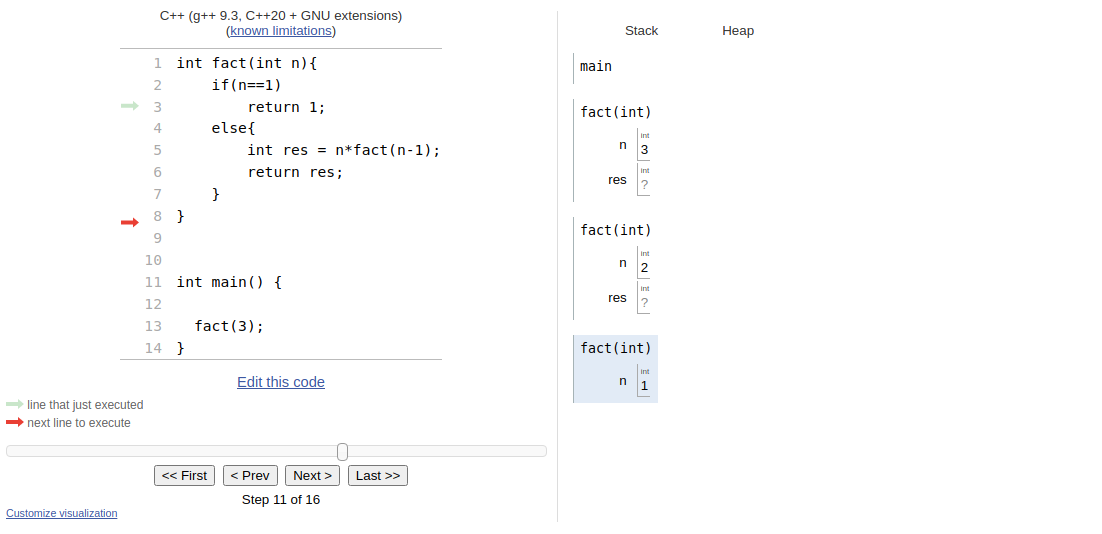
\includegraphics[scale=0.5]{images/pythontutor.png}
\caption{site pythontutor.com}
\end{figure}

\begin{exemplo}
O algoritmo de Euclides é um algoritmo que foi descrito no seu livro Elementos (300 A.C). O problema original era encontrar a maior medida comum capaz de medir dois comprimentos BA e DC. 

A Figura \ref{fig::euclides} ilustra o processo sugerido por Euclides para encontrar o maior medida comum de dois comprimentos BA e DC. Inicialmente, você começa com dois comprimentos iniciais BA e DC, ambos definidos como múltiplos de uma unidade de comprimento comum. Queremos encontrar o valor do maior comprimento capaz de medir os dois comprimentos. Inicialmente, tentamos medir o comprimento BA usando o comprimento DC. Nesse processo de medição, obtemos uma sobra que vale EA. Nesse momento, podemos perceber que se encontramos uma medida que mede EA e DC, podemos usar a mesma medida para medir BA e DC.

Aplicado aos números naturais, o algoritmo de Euclides para encontrar o máximo dividor comum de $a$ e $b$, denotado por mdc(a,b), pode ser definido  recursivamente  da seguinte maneira:

\begin{itemize}
    \item $mdc(a, b) = a$, se $b=0$
    \item $mdc(a, b) = mdc(b, a \mod b)$, caso contrário. 
\end{itemize}

\end{exemplo}


\begin{figure}[!h]
\label{fig::euclides}
\centering
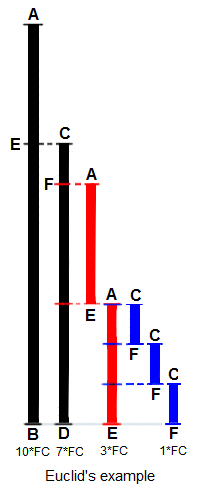
\includegraphics[scale=0.5]{images/Euclid Example.png}
\caption{Algoritmo de Euclides}
\end{figure}


O algoritmo recursivo para calcular o máximo divisor comum de $a$ e $b$ é: 

\begin{minted}{C++}
int mdc(int a, int b){
	if(b==0) return a;
	else return mdc(b, a%b);
}
\end{minted}

\begin{exemplo}
O algoritmo binário do máximo divisor comum foi publicado pelo físico e programador Josef Stein em 1967, mas pode ter sido conhecido no século II AC, na China Antiga.

A Figura \ref{fig::binarygcd} mostra a visualização geométrica do algoritmo binário do máximo divisor comum. O algoritmo binário do máximo divisor comum de $a$ e $b$ pode ser descrito pelas seguintes regras:

\begin{itemize}
    \item mdc(a, 0) = a
    \item mdc(0, b) = b
    \item mdc(2u, 2v) = mdc(u,v)
    \item mdc(2u, v) = mdc(u,v), se v é ímpar.
    \item mdc(u, 2v) = mdc(u,v), se u é ímpar.
    \item mdc(u, v) = mdc(|u-v|, min(u,v) ), se u e v são ímpares
    
\end{itemize}


\end{exemplo}


\begin{figure}[!h]
\label{fig::binarygcd}
\centering
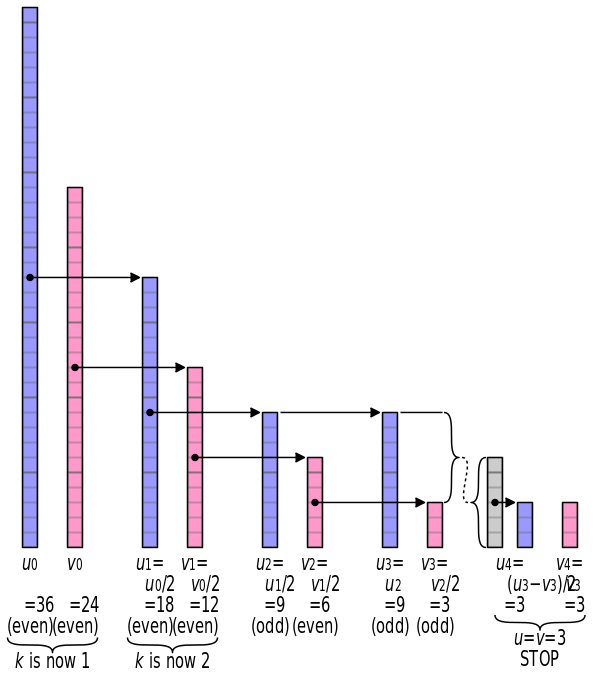
\includegraphics[scale=0.5]{images/Binary_GCD_algorithm_visualisation.svg.png}
\caption{Algoritmo de Euclides}
\end{figure}


Uma implementação do algoritmo binário do máximo divisor comum em C++:
\begin{minted}{C++}
int binarygcd(int a, int b){
    if(b == 0) return a;
    if(a == 0) return b;
    if( a % 2 == 0){
        if( b%2 == 0){
            return 2*binarygcd(a/2, b/2);
        }else{
            return binarygcd(a/2, b);
        }
    }else{
        if( b%2 == 0){
            return binarygcd(a, b/2);
        }else{
            return binarygcd( abs(a-b), min(a,b));
        }
    }

}
\end{minted}



